% HW1 for Intro to Data Science
% also my first real foray into LaTeX ._.

\documentclass{article} 
\usepackage{fancyhdr, titling, graphicx, mathtools, fixltx2e}
\pagestyle{fancy}

% put name and page number in header
\fancyhead[L]{Green, Ben}
\fancyhead[R]{Page \thepage}

\author{Ben Green}
\title{Intro to Data Science HW 1}

\begin{document}

% title page
\begin{titlepage}
	\begin{center}
	\textsc{\LARGE Intro to Data Science HW 1}\\
	\vspace{3mm}
	
	{\large \theauthor}\\
	
	\tableofcontents
	\setcounter{secnumdepth}{0}
	\vfill
	
	{\large \today}
	\end{center}

\end{titlepage}

\section{Question 1}

\subsection{1a.}
\begin{table}[h]
\begin{center}
\begin{tabular}{ll}
Feature Name                                    & Feature Type                  \\ \hline
\multicolumn{1}{|l|}{\texttt{producer}}                  & \multicolumn{1}{l|}{nominal}  \\ \hline
\multicolumn{1}{|l|}{\texttt{release\_to\_review\_time}} & \multicolumn{1}{l|}{interval} \\ \hline
\multicolumn{1}{|l|}{\texttt{used\_real\_name}}          & \multicolumn{1}{l|}{binary}   \\ \hline
\multicolumn{1}{|l|}{\texttt{verified\_purchase}}        & \multicolumn{1}{l|}{binary}   \\ \hline
\multicolumn{1}{|l|}{\texttt{rating}}                    & \multicolumn{1}{l|}{{ordinal}}  \\ \hline
\multicolumn{1}{|l|}{\texttt{helpfulness}}               & \multicolumn{1}{l|}{ratio}  \\ \hline
\multicolumn{1}{|l|}{\texttt{number\_of\_votes}}         & \multicolumn{1}{l|}{ratio}    \\ \hline
\multicolumn{1}{|l|}{\texttt{length\_of\_review\_text}}  & \multicolumn{1}{l|}{ratio}    \\ \hline
\end{tabular}
\end{center}
\end{table}

\subsection{1b.}
The mode of \texttt{producer} is Apple, with 4480 entries.

\subsection{1c.}
5077/9585, or 53\% of reviewers used their real name and had a verified purchase.

\subsection{1d.}
5077/13989, or 36\% of reviews with a verified purchase had a reviewer who used their real name.

\subsection{1e.}
\begin{table}[h]
\begin{center}
\begin{tabular}{|l|l|}
\hline
\textbf{Measure} & \textbf{Value} \\ \hline
min              & -537           \\ \hline
q1               & 74             \\ \hline
median           & 144            \\ \hline
q3				 & 290			  \\ \hline
max              & 11686          \\ \hline
interquartile    & 215            \\ \hline
\end{tabular}
\end{center}
\end{table}
These numbers can be displayed conveniently in a boxplot.

\subsection{1f.} 
\begin{center}
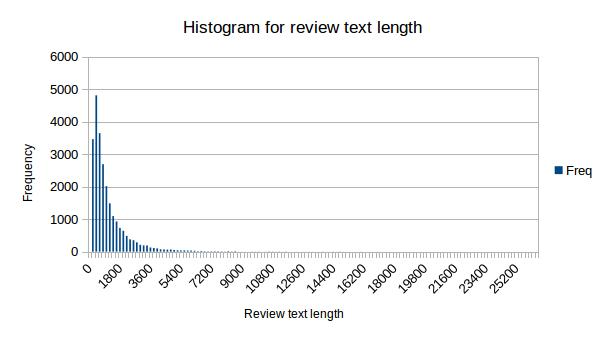
\includegraphics[keepaspectratio, scale=0.5]{histogram2.jpg}
\end{center}

\subsection{1g.}
Yes, the distribution of \texttt{length\_of\_review\_text}  is heavily skewed towards the shorter end. There are outliers of 18275, 22492, and 26332.

\subsection{1h.}
The Pearson correlation value between \texttt{length\_of\_review\_text} and \texttt{helpfulness} is approximately .25. This indicates that there is a slight positive correlation between these two variables.

\subsection{1i.}
\begin{center}
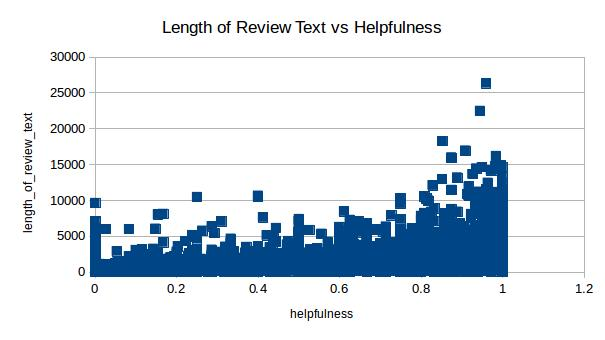
\includegraphics[keepaspectratio, scale=0.5]{scatter.jpg}
\end{center}

\section{Question 2}
Regarding the AND construction, \emph{r} = 3 being the number of hash functions and the LSH family \{d1,d2,0.6,0.4\}, the new family that is derived is:

\begin{center}
 \{d1,d2,0.6\textsuperscript{3},0.4\textsuperscript{3}\}\vspace{2mm}\\
\noindent\emph{w} =.216\\
\emph{x} =.064\\
\end{center}


\noindent Regarding the OR construction, \emph{r} = 3 being number of hash functions and the LSH family \{d1,d2,.216,0.64\}, the new family that is derived is:

\begin{center}
\{d1,d2,1-(1-(0.6))\textsuperscript3,1-(1-(0.4))\textsuperscript3\}\vspace{2mm}\\
\noindent \emph{y} = 0.936\\
\emph{z} = 0.784
\end{center}


\section{Question 3}

\subsection{3a.}
Sketch of vector \emph{u} = [1.25, -1.75, 1.75]\\
Sketch of vector \emph{v} = [0.95, -0.95, 1.35]\\
Sketch of vector \emph{w} = [-0.35, 1.65, 1.85]\\
\\The sketches were constructed by taking the dot products of each vector with each randomly generated vector.

\subsection{3b.}
\begin{equation}
\frac{u \cdot v}{\|u\| \cdot \|v\|} = 0.949
\end{equation}
\vspace{3mm}
\begin{equation}
\frac{u \cdot w}{\|u\| \cdot \|w\|} = 0.017
\end{equation}

\section{Question 4}

\subsection{4a.}
The Mahalanobis distance reduces to the Euclidian distance when the covariance matrix is the identity matrix.

\subsection{4b.}
The Mahalanobis distance reduces to the Euclidian distance when the covariance matrix is a diagonal matrix.

\section{Question 5}

\subsection{5a.}
The minihash signatures for each column are as follows:

\begin{table}[h]
\begin{tabular}{|l|l|l|l|l|}
\hline
\textbf{\emph{S}\textsubscript{1}} & \textbf{\emph{S}\textsubscript{2}} & \textbf{\emph{S}\textsubscript{3}} & \textbf{\emph{S}\textsubscript{4}} & \textbf{\emph{S}\textsubscript{5}} \\ \hline
5           & 5           & 1           & 1           & 1           \\ \hline
5           & 2           & 2           & 2           & 2           \\ \hline
3           & 0           & 1           & 4           & 0           \\ \hline
\end{tabular}
\end{table}

\subsection{5b.}
Only h\textsubscript{2} is a true permutation.

\subsection{5c.}

Estimated Jaccard Similarities:
\begin{table}[h]
\begin{tabular}{|l|l|l|l|l|l|}
\hline
\textbf{1-2} & \textbf{1-3} & \textbf{1-4} & \textbf{2-3} & \textbf{2-4} & \textbf{S6} \\ \hline
0            & 0            & 1/4          & 0            & 1/4          & 1/4         \\ \hline
\end{tabular}
\end{table}\\
True Jaccard Similarities:
\begin{table}[h]
\begin{tabular}{|l|l|l|l|l|l|}
\hline
\textbf{1-2} & \textbf{1-3} & \textbf{1-4} & \textbf{2-3} & \textbf{2-4} & \textbf{S6} \\ \hline
1/3          & 1/3          & 1/3          & 2/3          & 2/3          & 2/3         \\ \hline
\end{tabular}
\end{table}

\section{Question 6}
The stop-word based shingles for the sentences are:\\

\{and Mrs.Dursley, of number four, to say that, that they were\}\vspace{2mm}

\{for the first, the first time, an argument had, at number four\}\\

\noindent There are no matches between shingles of each sentence, so the Jaccard Similarity is 0/8.

\section{Question 7}

The logit function can be used to transform values obtained from a logistic equation to generate a sequence of random numbers with an (almost) normal distribution.

\end{document}